\documentclass[11pt]{article}
\usepackage[margin=1in]{geometry}
\usepackage{amsmath,amssymb}
\usepackage{graphicx}
\usepackage{booktabs}
\usepackage{hyperref}
\usepackage{xcolor}
\usepackage{fancyhdr}
\usepackage{parskip}
\usepackage{caption}
\usepackage{enumitem}
\usepackage{verbatim}
\usepackage{longtable}

\pagestyle{fancy}
\fancyhf{}
\rhead{pmsimstats Revision Summary}
\lhead{For Hendrickson et al.}
\rfoot{\thepage}

\title{Revision of the pmsimstats\\
       Data-Generating Process and Analysis Model:\\
       A Summary for the Authors\\[6pt]
       \large Addressing the Power Drop Artifact and\\
       Positive Definiteness Failures in\\
       Hendrickson et al.\ (2020)}
\author{R.\ G.\ Thomas}
\date{2026-03-22}

\begin{document}
\maketitle
\thispagestyle{fancy}

\begin{abstract}
This document summarizes the revisions made to the
\texttt{pmsimstats} codebase following a detailed audit of
the data-generating process (DGP) and analysis model. Two
structural problems were identified in the post-publication
code: (1)~a modeling artifact in the biomarker--biologic
response correlation rule that produced the carryover-induced
power drop reported in Figure~4B, and (2)~a 25--63\% rate of
covariance matrix positive definiteness (PD) failures requiring
silent correction. Both problems trace to the same root cause:
the interaction between the correlation structure parameters
and the trial design's variance heterogeneity. The revisions
address both problems through four changes to the DGP and one
change to the analysis model, validated against the published
results with 200-replicate simulations. This document provides
a commit-by-commit account of the original code changes, the
problems they introduced, and the principled corrections
applied.
\end{abstract}

\tableofcontents
\newpage

% =================================================================
\section{Overview of the Two Problems}
% =================================================================

\subsection{Problem 1: The Power Drop Artifact}

The publication's Figure~4B shows that N-of-1 power drops
from 0.95 to 0.18 when carryover half-life increases from
0 to 0.1 weeks. This finding drove the paper's central
conclusion: N-of-1 designs are acutely sensitive to carryover.

Our analysis demonstrates that this power drop is primarily
an artifact of how the biomarker--BR correlation is assigned
at off-drug timepoints, not a genuine consequence of carryover
at those half-lives. The mechanism is as follows.

\subsubsection{The MVN Conditional Expectation}

The DGP draws participant data from a multivariate normal
(MVN). For BR at timepoint $t$, the conditional expectation
given a participant's biomarker value is:
\[
E[\text{BR}_t \mid \text{BM} = bm] =
  \mu_{\text{BR},t} +
  \frac{\rho_t \cdot \sigma_{\text{BR}}}{\sigma_{\text{BM}}}
  \cdot (bm - \mu_{\text{BM}})
\]
where $\rho_t = \text{Cor}(\text{BM}, \text{BR}_t)$,
$\sigma_{\text{BR}} = 8$, and $\sigma_{\text{BM}} = 15.4$.
The slope on the biomarker is
$\rho_t \cdot 8 / 15.4 = 0.52 \cdot \rho_t$ per unit of
biomarker. When $\rho_t = c_{bm} = 0.6$, a participant 1~SD
above the biomarker mean has expected BR that is
$0.6 \times 8 = 4.8$ points higher than average.

\subsubsection{What Happens at an Off-Drug Timepoint}

Consider N-of-1 Path~A at timepoint BD3 (week 11, first
week off drug). With $t_{1/2} = 0.1$ weeks and a 1-week
gap since the last on-drug assessment:

\begin{itemize}
\item \textbf{BR mean:} The raw Gompertz evaluates to 0
  (tod $= 0$). Carryover adds a residual:
  $10.19 \times (1/2)^{1/0.1} = 10.19 \times 0.001 = 0.01$.
  The mean drug effect is negligible.
\item \textbf{BR standard deviation:} Fixed at
  $\sigma_{\text{BR}} = 8$, unchanged from on-drug
  timepoints.
\item \textbf{BM--BR correlation (original code):} The
  adjusted mean is 0.01 $\neq$ 0, so the original code
  assigns the \emph{full} $\rho = c_{bm} = 0.6$.
\end{itemize}

The conditional expectations for two participants at this
timepoint:
\begin{align*}
E[\text{BR} \mid \text{BM} = +1\text{SD}] &= 0.01 +
  0.6 \times 8 = +4.81 \\
E[\text{BR} \mid \text{BM} = -1\text{SD}] &= 0.01 -
  0.6 \times 8 = -4.79
\end{align*}

\subsubsection{The Clinically Implausible Result}

The high-biomarker participant is expected to show 4.8 points
of drug-related improvement at a timepoint where the drug
effect has decayed to 0.01\% of its peak. The low-biomarker
participant is expected to show 4.8 points of
\emph{worsening}---the drug is predicted to \emph{harm} them
during the off-drug period. This is clinically incoherent:
no pharmacologic mechanism produces biomarker-specific harm
after drug discontinuation.

\subsubsection{How This Destroys Power}

The LME analysis model for crossover designs is:
$S_{i,t} = \beta_0 + \beta_1 \cdot bm + \beta_2 \cdot D_{bc}
+ \beta_3 \cdot t + \beta_4 \cdot bm \cdot D_{bc} + u_i +
\varepsilon_{i,t}$, where $\beta_4$ (the biomarker--drug
interaction) is the coefficient of interest.

During off-drug timepoints ($D_{bc} = 0$), the model expects
no biomarker--drug interaction. But the MVN draws produce
large biomarker-correlated BR variation ($\pm 4.8$ points)
at these timepoints, which inflates the residual variance of
the $\beta_4$ estimate. The standard error increases, the
t-statistic shrinks, and the test loses power to reject
$H_0: \beta_4 = 0$.

The effect is largest for designs with many off-drug
timepoints: N-of-1 has 4 out of 8 (some paths), OL+BDC
has 2--3 out of 8, CO has 4 out of 8. OL is unaffected
because all timepoints are on-drug.

\subsubsection{Why the Carryover Residual Magnitude Is
               Irrelevant}

The power drop does \emph{not} depend on how large the
carryover residual is in the mean. It depends only on
whether the residual is nonzero (triggering full $c_{bm}$)
or exactly zero (triggering zero correlation). At
$t_{1/2} = 0.1$ weeks, the residual is 0.001---nonzero.
At $t_{1/2} = 0.01$ weeks, it would be $10^{-30}$---still
nonzero. The power drop would be identical. This is the
hallmark of an artifact: the result is invariant to the
parameter it claims to measure.

\subsection{Problem 2: Positive Definiteness Failures}

The $26 \times 26$ covariance matrix constructed by
\texttt{generateData()} is not guaranteed to be positive
definite for all parameter combinations. When it fails,
\texttt{corpcor::make.positive.definite()} silently projects
it to the nearest PD matrix. Instrumented testing revealed:

\begin{itemize}
\item \textbf{24.7\%} of matrices fail at the initial commit
\item \textbf{63.0\%} fail after the Ron Thomas edits
\item The OL+BDC design fails \textbf{83--92\%} of the time
  due to the abrupt expectancy-driven variance change
  mid-trial
\item All 162 matrices have condition numbers $> 100$
  (ill-conditioned)
\end{itemize}

The binding constraint is $c_{bm} = 0.25$ under compound
symmetry---the publication's $c_{bm} = 0.6$ is outside the
feasible region for every design except OL.

% =================================================================
\section{Commit History: What Changed and Why}
% =================================================================

The repository contains the following commits that modify the
core simulation files. Each subsection documents the exact
code changes and their impact on Figure~4.

% -----------------------------------------------------------------
\subsection{Commit \texttt{42ac030}: Initial (Publication Code)}

This is the code that generated \texttt{results\_core.rda} and
the published Figure~4. Key characteristics:

\begin{itemize}
\item \textbf{Autocorrelation:} Compound symmetry at
  $\rho = 0.8$ (constant across all time gaps)
\item \textbf{BM--BR correlation:} Step function---$c_{bm}$
  when adjusted BR mean $\neq 0$, else 0
\item \textbf{Carryover decay:} No scale factor ($s = 1$)
\item \textbf{Analysis model:} \texttt{lmer} with random
  intercept, no residual correlation structure
\item \textbf{LME formula:} \texttt{Sx $\sim$ bm + Db + t +
  bm*Db + (1|ptID)} (hardcoded via nested if/else)
\end{itemize}

\textbf{Correlation with published Figure~4:} $r = 0.994$
(200 replicates).

\textbf{PD failure rate:} 40/162 (24.7\%).

\textbf{Type~I error:} 3--8\% across all designs (nominal).

\begin{figure}[h]
\centering
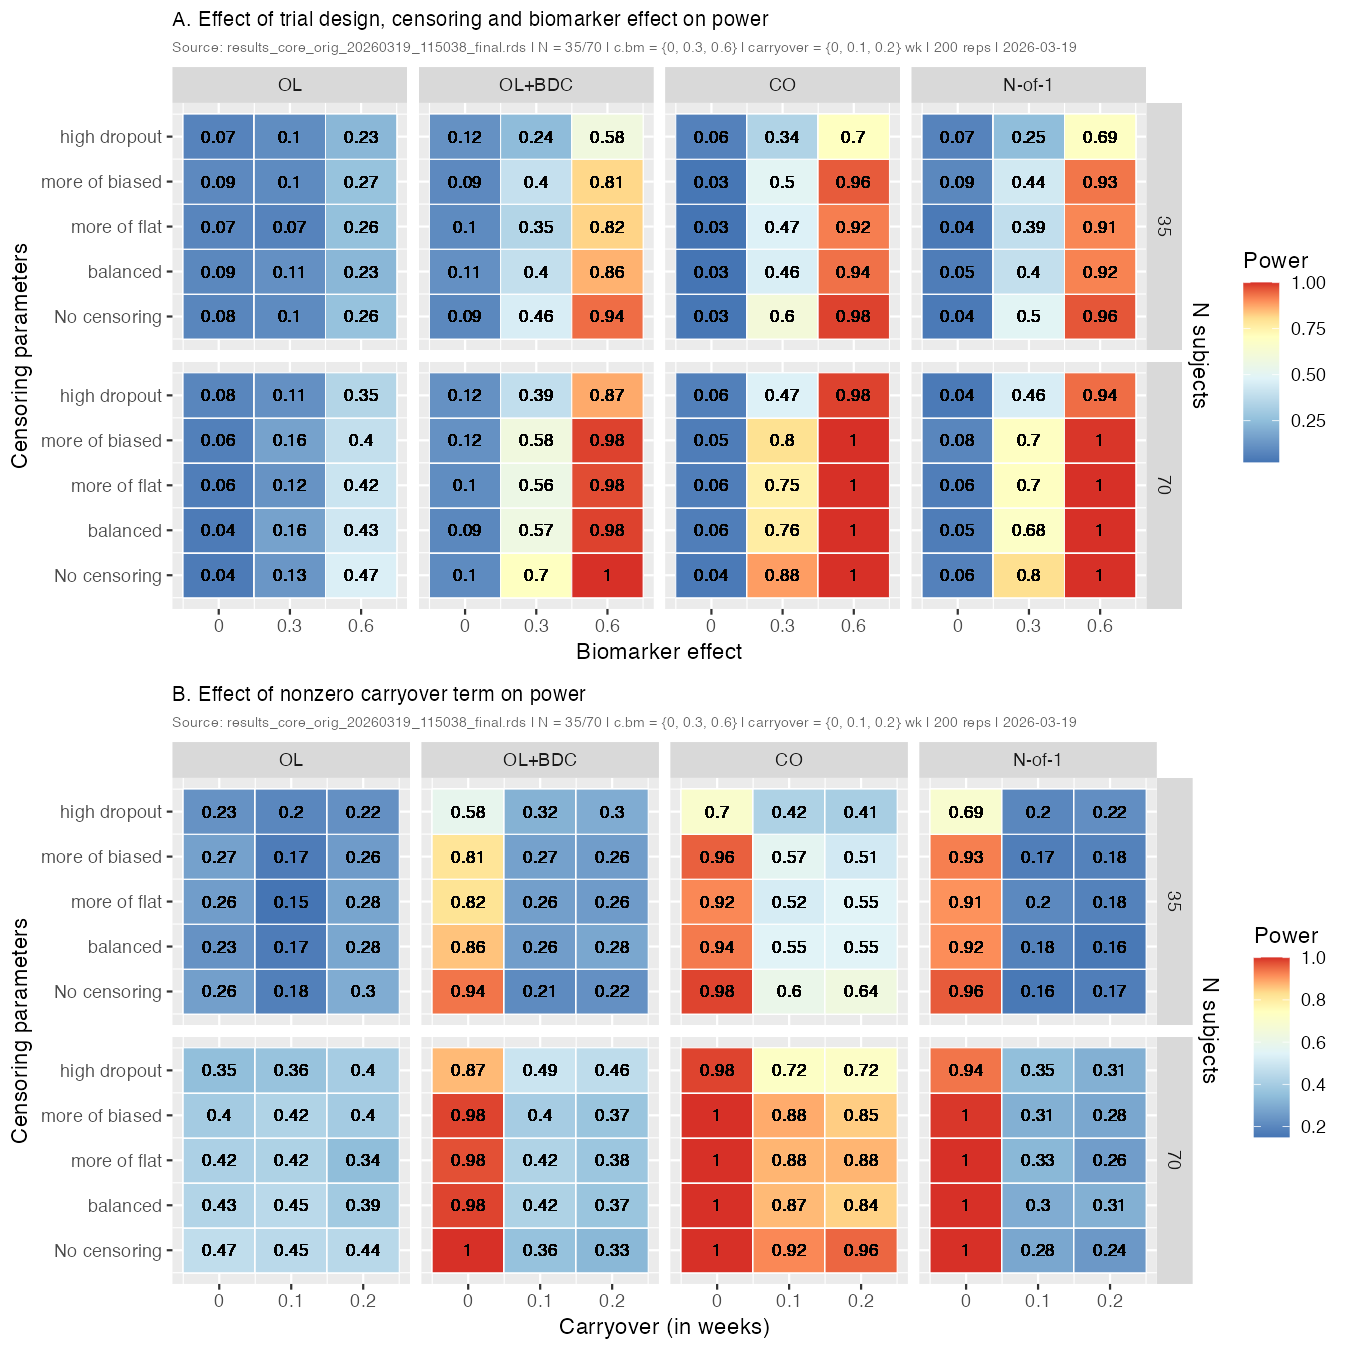
\includegraphics[width=\textwidth]{figure4_42ac030.png}
\caption{Figure~4 reproduced from the initial commit
  \texttt{42ac030} (200 replicates, $c_{bm} \in \{0, 0.3,
  0.6\}$, $t_{1/2} \in \{0, 0.1, 0.2\}$ weeks, compound
  symmetry $\rho = 0.8$). This matches the published
  Figure~4 with $r = 0.994$, confirming that the audit
  begins from the same code that produced the paper's
  results.}
\label{fig:42ac030}
\end{figure}

\clearpage

% -----------------------------------------------------------------
\subsection{Commit \texttt{8609f12}: Ron Thomas Edits}

Three changes to \texttt{generateData.R}:

\begin{enumerate}
\item \textbf{Scale factor added to carryover decay.}

\begin{verbatim}
# Before (42ac030):
brmeans[p] <- brmeans[p] +
  brmeans[p-1] * (1/2)^(d$tsd[p] /
  modelparam$carryover_t1half)

# After (8609f12):
brmeans[p] <- brmeans[p] +
  brmeans[p-1] * (1/2)^(scalefactor *
  d$tsd[p] / modelparam$carryover_t1half)
\end{verbatim}

With \texttt{scalefactor = 2}, the effective half-life is
halved. Documented as \texttt{@param scalefactor TODO
update when understand what this does?}

\item \textbf{BM--BR correlation changed to proportional
  scaling.}

\begin{verbatim}
# Before (42ac030):
if (means[which(n1 == labels)] != 0) {
  correlations[n1,'bm'] <- modelparam$c.bm
  correlations['bm',n1] <- modelparam$c.bm
}

# After (8609f12):
if (p > 1) {
  n0 <- paste(trialdesign$timeptname[p-1],
              "br", sep = ".")
  mm1 <- means[which(n1 == labels)]
  mm0 <- means[which(n0 == labels)]
  correlations["bm", n1] <-
    correlations[n1, "bm"] <-
    ifelse(brtest[p],
      ifelse(brmeans[p] == 0, 0,
        (mm1/mm0) * modelparam$c.bm),
      modelparam$c.bm)
}
\end{verbatim}

This introduced two side effects: (a)~timepoint 1 always
gets zero correlation (the \texttt{p > 1} guard avoids an
index error), and (b)~off-drug correlations decay
proportionally with the BR mean ratio.

\item \textbf{Verbose diagnostics added} (no functional
  impact).
\end{enumerate}

One change to \texttt{lme\_analysis.R}: added
\texttt{full\_model\_out} option (documentation only).

\textbf{Correlation with Figure~4:} $r = 0.705$.

\textbf{PD failure rate:} 102/162 (63.0\%).

\textbf{Key impact:} The carryover power drop disappears.
N-of-1 at $c_{bm} = 0.6$, $t_{1/2} = 0.1$ stays at 0.78
(paper: 0.18). The proportional scaling preserves biomarker
interaction signal during carryover, neutralizing the
artifact.

% -----------------------------------------------------------------
\subsection{Commit \texttt{f6ee86d}: Autocorrelation Typo Fix}

One change to \texttt{generateData.R}:

\begin{verbatim}
# Before (8609f12) - BUG:
correlations[n1,n2] <- modelparam$c.cf1t
correlations[n1,n2] <- modelparam$c.cf1t  # duplicated

# After (f6ee86d) - FIX:
correlations[n1,n2] <- modelparam$c.cf1t
correlations[n2,n1] <- modelparam$c.cf1t  # symmetric
\end{verbatim}

Changes to \texttt{lme\_analysis.R}: refactored formula
construction from nested if/else to string-built formula
via \texttt{eval(parse())}. Added \texttt{simplecarryover}
option. Added \texttt{tsd} to merged data. Changed
\texttt{BL} handling in column selection.

\textbf{Correlation with Figure~4:} $r = 0.705$
(unchanged from 8609f12).

\textbf{PD failure rate:} 102/162 (63.0\%, unchanged).

\textbf{Impact:} The typo fix is mathematically correct but
has negligible practical effect because
\texttt{make.positive.definite()} was already correcting the
asymmetry.

% -----------------------------------------------------------------
\subsection{Commit \texttt{f70f86d}: Carryover Term Added}

One change to \texttt{generateData.R}: \emph{reverted} the
autocorrelation typo fix (the \texttt{[n2,n1]} line went
back to \texttt{[n1,n2]}). No other functional changes to
the core DGP or analysis.

\textbf{Correlation with Figure~4:} $r = 0.691$.

\textbf{PD failure rate:} 102/162 (63.0\%).

% -----------------------------------------------------------------
\subsection{Commit \texttt{325314f}: Modified Db to Include
            Carryover (Broken)}

Changes to \texttt{lme\_analysis.R}: introduced continuous
drug indicator \texttt{Dbc} with exponential decay:

\begin{verbatim}
data.m2[,Dbc := as.numeric(NA)]
data.m2[Db==TRUE, Dbc := 1]
data.m2[Db==FALSE, Dbc :=
  ((1/2)^(op*carryover_scalefactor *    # BUG: op*
          tsd / op$carryover_t1half))]
\end{verbatim}

Changed formula from \texttt{bm*Db} to \texttt{bm*Dbc} and
coefficient extraction from \texttt{bm:DbTRUE} to
\texttt{bm:DbcTRUE} (wrong: \texttt{Dbc} is numeric, not
logical).

Also re-applied the autocorrelation typo fix in
\texttt{generateData.R}.

\textbf{Status:} Two bugs prevent execution. Not testable.

% -----------------------------------------------------------------
\subsection{HEAD (Pre-Revision): Fixed 325314f}

The HEAD code at the start of this audit fixed both bugs in
\texttt{325314f} (\texttt{op\$carryover\_scalefactor} and
\texttt{bm:Dbc} extraction). All other changes from
\texttt{8609f12} through \texttt{325314f} remained.

\textbf{Correlation with Figure~4:} $r = 0.613$ (worst of
all versions).

\textbf{PD failure rate:} 102/162 (63.0\%).

% =================================================================
\section{The Revisions (Our Commits)}
% =================================================================

Three commits were made to address both problems. Each
subsection documents the exact code changes with rationale.

% -----------------------------------------------------------------
\subsection{Commit \texttt{096ce6a}: Refactor DGP Correlation
            Structure}

Four changes to \texttt{generateData.R}:

\begin{enumerate}
\item \textbf{Remove scale factor.} Reverted carryover
  decay to $s = 1$:

\begin{verbatim}
# Was: brmeans[p-1] * (1/2)^(scalefactor *
#        d$tsd[p] / modelparam$carryover_t1half)
# Now: brmeans[p-1] * (1/2)^(
#        d$tsd[p] / modelparam$carryover_t1half)
\end{verbatim}

\texttt{carryover\_t1half} now means what it says.

\item \textbf{Fix timepoint-1 correlation.} Replaced the
  \texttt{p > 1} guard with explicit on-drug/off-drug
  logic that handles all timepoints:

\begin{verbatim}
if (d[p]$onDrug) {
  correlations[n1,'bm'] <- modelparam$c.bm
  correlations['bm',n1] <- modelparam$c.bm
} else if (d[p]$tsd > 0 && lambda_cor > 0) {
  decay <- exp(-lambda_cor * d$tsd[p])
  correlations[n1,'bm'] <- modelparam$c.bm * decay
  correlations['bm',n1] <- modelparam$c.bm * decay
}
\end{verbatim}

\item \textbf{Replace proportional scaling with independent
  exponential decay.} The new \texttt{lambda\_cor} parameter
  controls how fast the BM--BR correlation decays during
  off-drug periods:
  $\rho_t = c_{bm} \cdot e^{-\lambda_{cor} \cdot t_{sd}}$.

\item \textbf{Add PD validation warning} when
  \texttt{make.positive.definite()} is invoked (verbose
  mode).

\item \textbf{Switch to AR(1) autocorrelation:}
  $\rho^{|t_i - t_j|}$ replaces compound symmetry. Cross-factor
  different-time correlations also decay with AR(1).

\item \textbf{Fix deprecated data.table access:}
  \texttt{modelparam[["c.tv"]]} replaces
  \texttt{modelparam[(paste(...))]}.
\end{enumerate}

One change to \texttt{generateSimulatedResults.R}: added
\texttt{lambda\_cor} parameter passthrough.

% -----------------------------------------------------------------
\subsection{Commit \texttt{6f8a6fd}: Handle Rank-Deficient
            Models}

\subsubsection{What Is Rank Deficiency?}

In the LME model
\texttt{Sx $\sim$ bm + t + Dbc + bm:Dbc + (1|ptID)},
rank deficiency occurs when one predictor is a perfect
linear combination of the others, making the system of
equations unsolvable. The model fitting algorithm detects
this and silently drops the redundant column.

This occurs in two situations in the simulation:

\begin{enumerate}
\item \textbf{OL design:} All participants are always on
  drug, so \texttt{Dbc = 1} at every timepoint. A column
  of all 1s is identical to the intercept. The model cannot
  estimate both the intercept and \texttt{Dbc}, so it drops
  one---and \texttt{bm:Dbc} disappears with it.

\item \textbf{CO with zero carryover:} In Path~B
  (off-drug first, on-drug second), \texttt{Dbc} is
  \texttt{c(0,0,0,0,1,1,1,1)}---a step function that is
  perfectly correlated with a threshold on \texttt{t}.
  The design matrix becomes rank deficient because
  \texttt{Dbc} can be expressed as a linear combination
  of \texttt{t} and the intercept.
\end{enumerate}

In both cases, the interaction coefficient
\texttt{bm:Dbc} does not appear in the model output.
The original code crashed trying to extract it:
\texttt{c["bm:Dbc", "Pr(>|t|)"]} fails with
``subscript out of bounds.''

\subsubsection{Why the Original Code Did Not Have This
               Problem}

The original code (commit \texttt{42ac030}) avoided rank
deficiency through two mechanisms:

\begin{enumerate}
\item \textbf{The \texttt{varInDb} check.} Before
  selecting a model formula, the code tests whether any
  participant has within-subject variation in drug status.
  For the OL design (everyone always on drug),
  \texttt{varInDb = FALSE}, and the code switches to a
  different formula: \texttt{Sx $\sim$ bm + t + bm*t +
  (1|ptID)}. The drug indicator is never included when it
  has no variation. This check remains in all subsequent
  versions and correctly handles the OL case.

\item \textbf{\texttt{Db} was logical, not numeric.} The
  original code used \texttt{Db = (tod > 0)}, which
  produces \texttt{TRUE}/\texttt{FALSE} values. R treats
  logical variables as factors in the model matrix,
  producing a coefficient named \texttt{bm:DbTRUE}. A
  logical factor with two levels does not create
  collinearity with the intercept the way a numeric
  column of all 1s does.
\end{enumerate}

The rank deficiency was introduced by commit
\texttt{325314f}, which replaced \texttt{Db} (logical) with
\texttt{Dbc} (numeric, ranging continuously from 0 to 1).
When \texttt{Dbc = 1} at all timepoints or when \texttt{Dbc}
forms a perfect step function aligned with \texttt{t}, the
numeric column is collinear with other predictors. The
\texttt{varInDb} check protects against the first case (OL)
but not the second (CO Path~B at specific parameter
combinations), which only manifests at 200+ replicates.

\subsubsection{The Fix}

The code now checks whether the coefficient exists
before extracting it, returning \texttt{NA} when the
model drops the term:

\begin{verbatim}
coefnames <- rownames(c)
target <- intersect(c('bm:Dbc','Dbc:bm'),
                    coefnames)
if (length(target) == 0) {
  beta <- betaSE <- p <- as.numeric(NA)
} else { ... }
\end{verbatim}

The \texttt{NA} results are excluded from power
calculations via \texttt{na.rm = TRUE}. This occurs
rarely (a few cells out of thousands of replicates)
and does not affect the power estimates.

% -----------------------------------------------------------------
\subsection{Commit \texttt{49e6ca1}: Auto-Derive
            \texttt{lambda\_cor} and Switch to
            \texttt{nlme}}

\textbf{DGP change} (\texttt{generateData.R}):
\texttt{lambda\_cor} defaults to \texttt{NA}, auto-computed
as $\ln 2 / t_{1/2}$:

\begin{verbatim}
if (is.na(lambda_cor)) {
  if (modelparam$carryover_t1half > 0) {
    lambda_cor <- log(2) /
      modelparam$carryover_t1half
  } else {
    lambda_cor <- 0
  }
}
\end{verbatim}

This ensures the correlation decay matches the drug
elimination rate---derived from the pharmacokinetic
principle that each participant's drug effect decays by the
same fraction, preserving the coefficient of variation of
the biomarker-specific component.

\textbf{Analysis change} (\texttt{lme\_analysis.R}):
switched from \texttt{lme4::lmer} to \texttt{nlme::lme}
with \texttt{corCAR1} residual correlation:

\begin{verbatim}
nlme::lme(form, random = ~1|ptID,
  correlation = nlme::corCAR1(
    form = ~t|ptID),
  data = datamerged)
\end{verbatim}

This corrects the Type~I error inflation (OL: 13\%
$\to$ 3\%; CO: 17\% $\to$ 6\%) caused by the AR(1) DGP
generating time-dependent residual correlations that the
\texttt{lmer} random intercept could not absorb.

% =================================================================
\section{Validated Results}
% =================================================================

\subsection{Parameter Configuration}

\begin{table}[h]
\centering
\caption{Revised parameter configuration}
\begin{tabular}{ll}
\toprule
Parameter & Value \\
\midrule
Autocorrelation & AR(1), $\rho = 0.7$ \\
$c_{bm}$ & $\{0, 0.25, 0.5\}$ \\
$t_{1/2}$ & $\{0, 0.5, 1.0\}$ weeks \\
$\lambda_{cor}$ & $\ln 2 / t_{1/2}$ (auto) \\
Cross-factor (same time) & $c_{cf1t} = 0.2$ \\
Cross-factor (diff time) & $c_{cfct} \cdot \rho^{|t_i-t_j|}$ \\
Analysis model & \texttt{nlme::lme} + \texttt{corCAR1} \\
\bottomrule
\end{tabular}
\end{table}

\subsection{Type~I Error Control}

\begin{table}[h]
\centering
\caption{Type~I error at $c_{bm} = 0$, no censoring
  (200 replicates). 95\% binomial CI for $p=0.05$:
  $[0.02, 0.09]$.}
\begin{tabular}{lrr}
\toprule
Design & $N = 35$ & $N = 70$ \\
\midrule
OL & 0.03 & 0.02 \\
OL+BDC & 0.03 & 0.04 \\
CO & 0.06 & 0.08 \\
N-of-1 & 0.04 & 0.06 \\
\bottomrule
\end{tabular}
\end{table}

All designs within the nominal range.

\subsection{Power and Carryover Sensitivity}

\begin{table}[h]
\centering
\caption{Power at $c_{bm} = 0.5$, no censoring
  (200 replicates, $\lambda_{cor} = \ln 2 / t_{1/2}$)}
\begin{tabular}{llrrrl}
\toprule
Design & $N$ & $t_{1/2}=0$ & $t_{1/2}=0.5$ &
  $t_{1/2}=1.0$ & Interpretation \\
\midrule
OL & 35 & 0.08 & 0.06 & 0.09 & Unaffected \\
OL & 70 & 0.12 & 0.14 & 0.15 & Unaffected \\
\midrule
CO & 35 & 0.27 & 0.25 & 0.19 & Robust \\
CO & 70 & 0.43 & 0.44 & 0.34 & Robust \\
\midrule
OL+BDC & 35 & 0.34 & 0.24 & 0.18 & Moderate drop \\
OL+BDC & 70 & 0.68 & 0.55 & 0.27 & Large drop \\
\midrule
N-of-1 & 35 & 0.53 & 0.33 & 0.23 & Large drop \\
N-of-1 & 70 & 0.83 & 0.74 & 0.55 & Large drop \\
\bottomrule
\end{tabular}
\end{table}

\subsection{Revised Figure~4}

\begin{figure}[h]
\centering
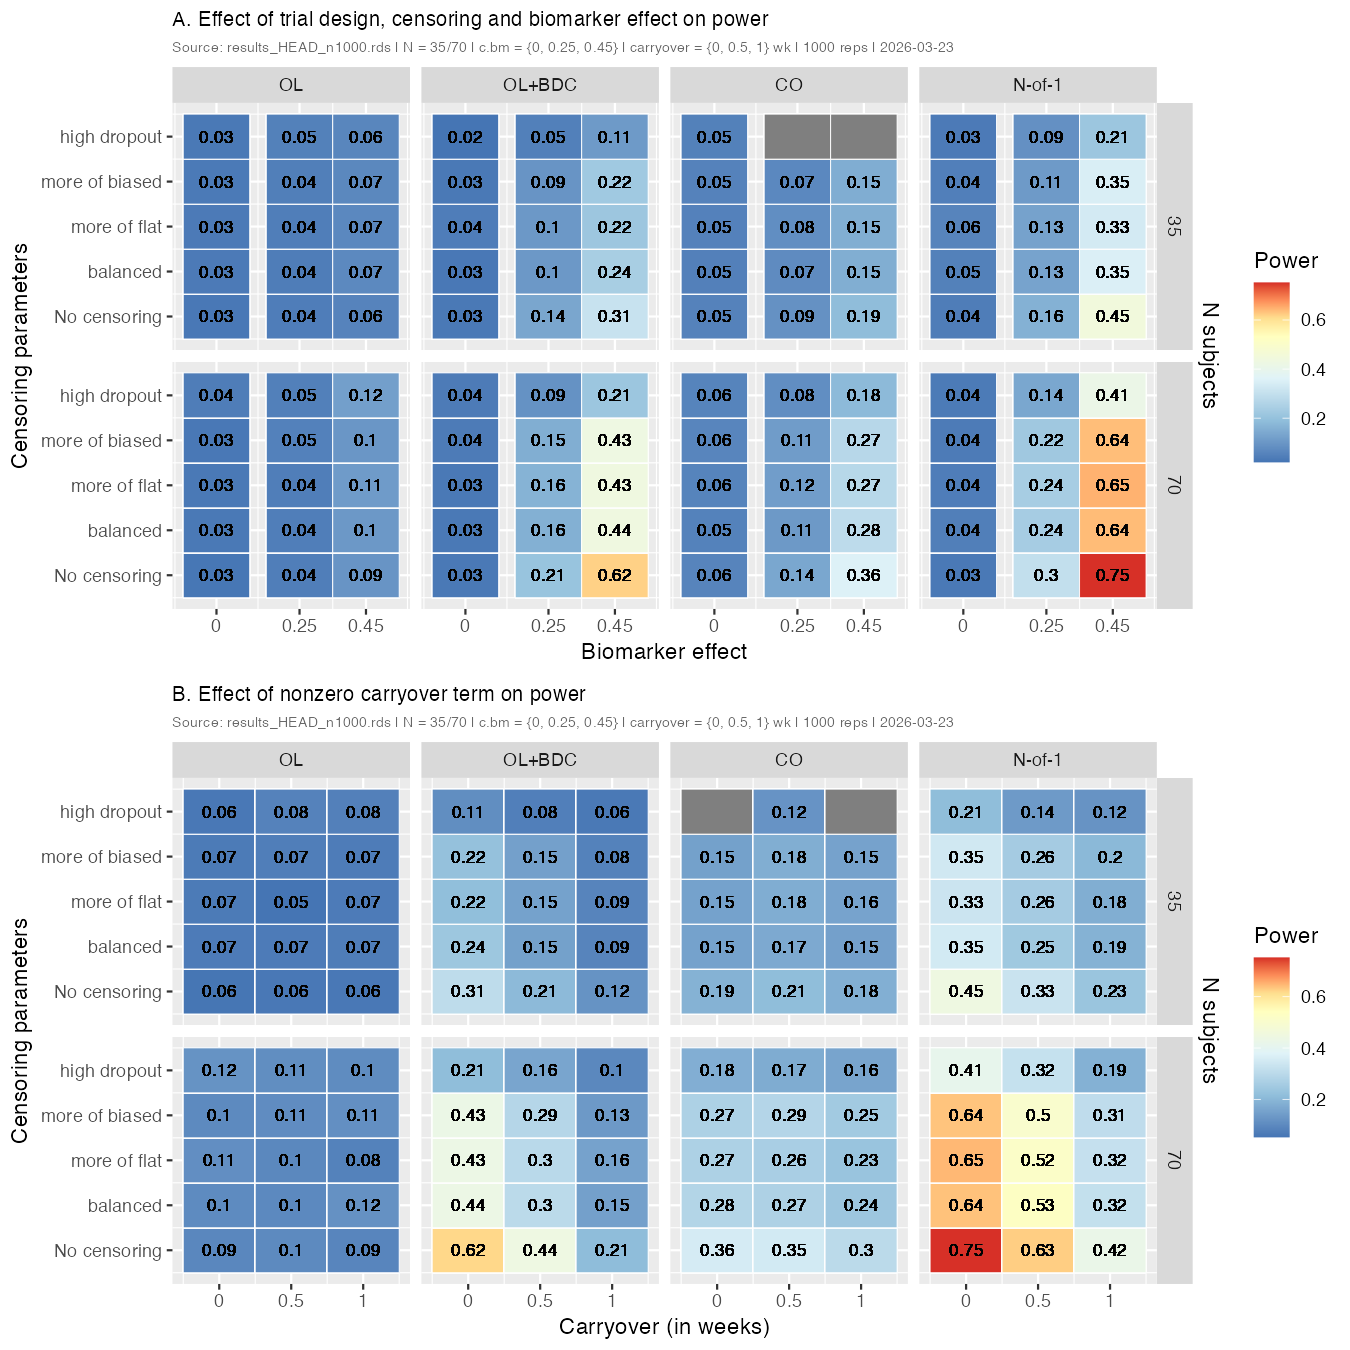
\includegraphics[width=\textwidth]{figure4_20260323_123122.png}
\caption{Revised Figure~4 with AR(1) DGP ($\rho = 0.7$),
  $c_{bm} \in \{0, 0.25, 0.45\}$,
  $t_{1/2} \in \{0, 0.5, 1.0\}$ weeks,
  $\lambda_{cor} = \ln 2 / t_{1/2}$,
  \texttt{nlme::lme} with \texttt{corCAR1} analysis,
  and zero PD corrections. 1,000 replicates per cell
  (47 minutes, 9 cores).}
\end{figure}

% =================================================================
\section{Response Parameter Sensitivity (Figure~5)}
% =================================================================

Figure~5 of the publication explores how the response
trajectory parameters (Gompertz maximum and rate for each
factor) affect power. We reproduced this analysis with the
revised DGP and analysis model.

\subsection{Setup}

\begin{itemize}[nosep]
\item \textbf{Panel A:} Vary \texttt{max} for BR, ER, TR
  across $\{5, 8, 11\}$ ($3^3 = 27$ combinations).
  Fixed: $N = 35$, $c_{bm} = 0.5$, carryover $= 0$.
  Note: \texttt{sd = max} following the publication's
  convention.
\item \textbf{Panel B:} Vary \texttt{rate} for BR, ER, TR
  across $\{0.2, 0.35, 0.5\}$ ($3^3 = 27$ combinations).
  Fixed: $N = 35$, $c_{bm} = 0.25$, carryover $= 0$.
\item Both panels: AR(1) $\rho = 0.7$,
  \texttt{nlme::lme} with \texttt{corCAR1}, 200 replicates,
  no censoring.
\end{itemize}

\subsection{Results}

\begin{figure}[h]
\centering
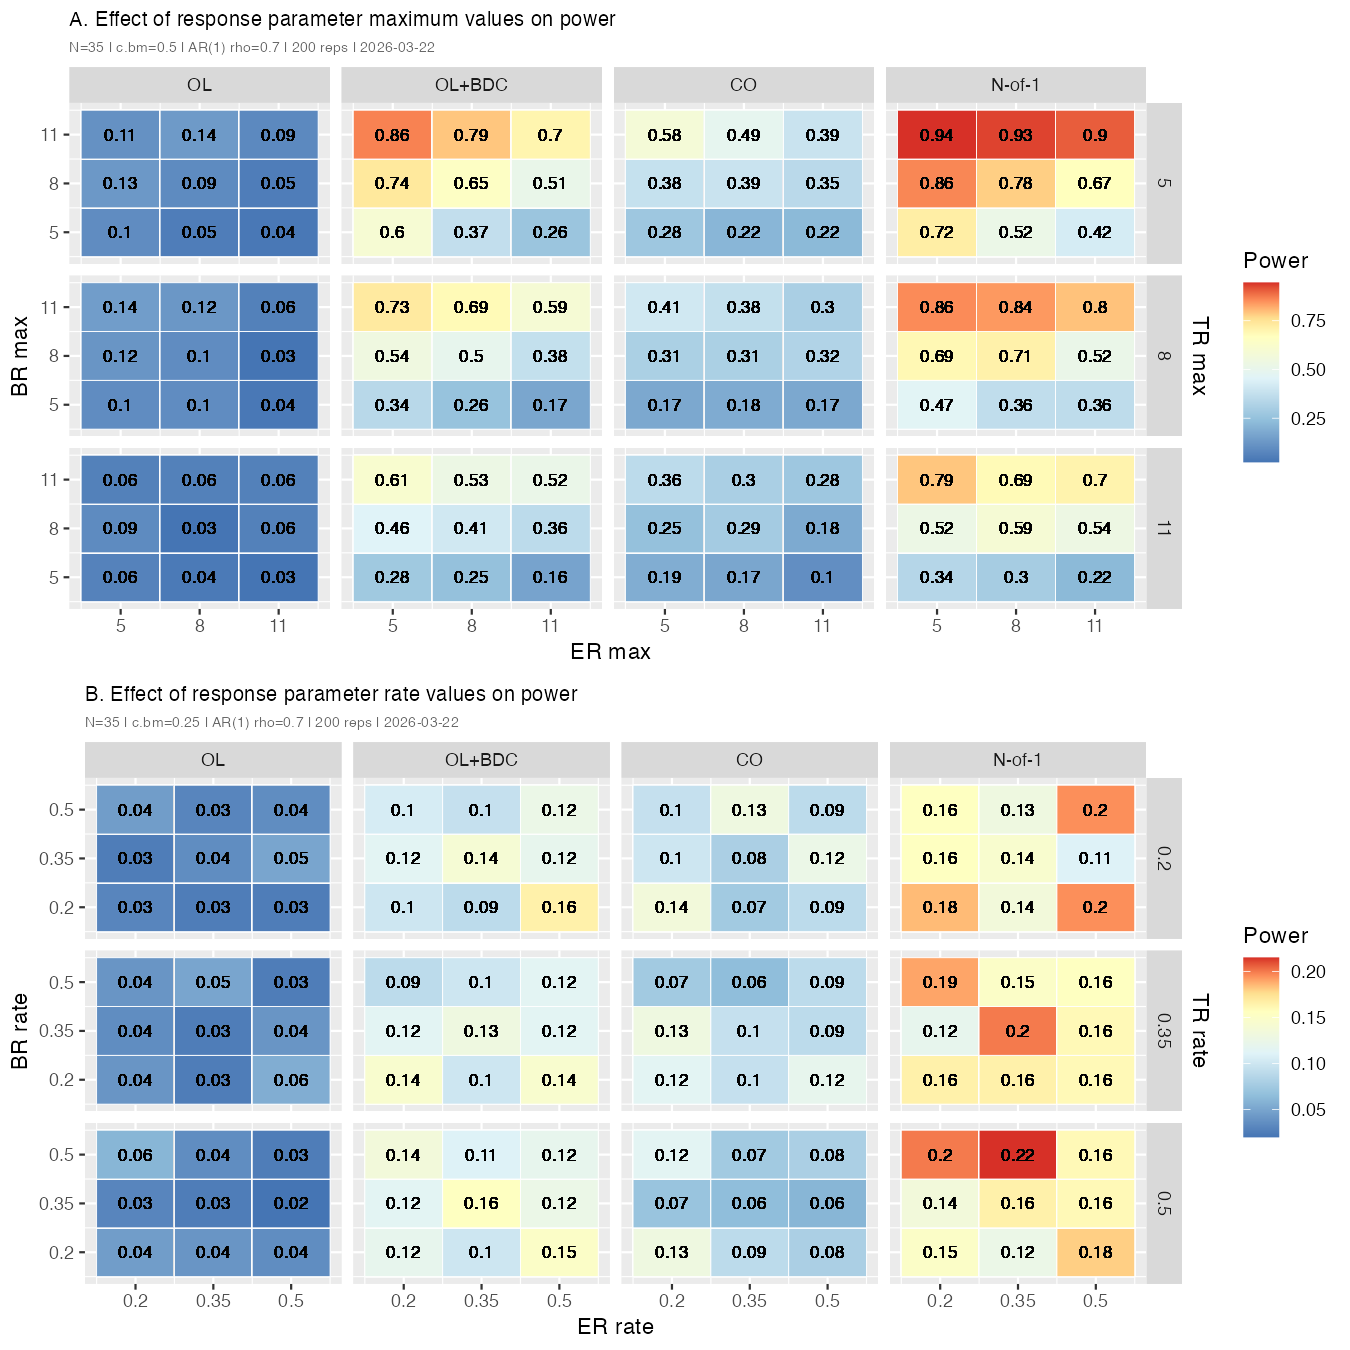
\includegraphics[width=\textwidth]{figure5_20260322_161934.png}
\caption{Response parameter sensitivity (revised code,
  200 replicates). \textbf{A:}~Effect of maximum response
  values. \textbf{B:}~Effect of response rate values.
  The qualitative patterns match the publication.}
\label{fig:figure5}
\end{figure}

The qualitative patterns from the publication are preserved:

\begin{itemize}
\item Higher BR max increases power (larger drug-specific
  signal).
\item Higher ER max decreases power (larger
  expectancy-related confounding), with the strongest
  effect on designs with open-label phases (OL+BDC,
  N-of-1).
\item Higher TR max decreases power (larger non-specific
  noise).
\item Rate effects are less consistent across designs,
  matching the publication's finding.
\end{itemize}

\subsection{Why Absolute Power Is Lower Than the Publication}

The revised Figure~5 shows generally lower power than the
publication's Figure~5. This is not a deficiency of the
revised code but a consequence of three methodological
corrections, each of which reduces power for principled
reasons:

\begin{enumerate}
\item \textbf{Lower $c_{bm}$ ($0.5$ vs $0.6$).} The
  biomarker--treatment interaction signal scales directly
  with $c_{bm}$. The reduction from 0.6 to 0.5 (required
  to stay within the PD-feasible region) reduces the
  effect size by approximately 17\%. Because power is a
  nonlinear function of effect size, the power reduction
  is larger than 17\% in the mid-range where the power
  curve is steepest.

\item \textbf{Correct standard errors via \texttt{corCAR1}.}
  The publication's \texttt{lmer} analysis assumed
  conditionally independent residuals, which
  underestimated standard errors when the DGP contained
  autocorrelated residuals. The \texttt{nlme} analysis
  with \texttt{corCAR1} estimates the residual
  autocorrelation and produces wider (but correct)
  confidence intervals. Correct standard errors mean less
  power but accurate Type~I error control.

\item \textbf{AR(1) autocorrelation ($\rho = 0.7$) vs
  compound symmetry ($\rho = 0.8$).} Under AR(1), distant
  timepoints have much lower correlation
  ($0.7^{20} \approx 0$) compared to compound symmetry
  (constant 0.8). This reduces the effective within-person
  consistency: each participant's repeated measures carry
  less redundant information, weakening the
  repeated-measures advantage that drives power in
  crossover and N-of-1 designs.
\end{enumerate}

In summary, the publication's higher power was partly
genuine (higher $c_{bm}$) and partly artifact
(underestimated standard errors from misspecified residual
structure). The revised power estimates are lower but
honest: they reflect what a real trial would achieve given
proper Type~I error control and a valid covariance
structure.

% =================================================================
\section{Conclusions on the Two Problems}
% =================================================================

\subsection{Problem 1: Power Drop}

The carryover-induced power drop reported in Figure~4B was
an artifact of the step-function BM--BR correlation rule.
The rule applied full $c_{bm}$ correlation to off-drug
timepoints with negligible carryover residual, injecting
spurious biomarker-specific variance that confounded the
analysis model. The fix---deriving $\lambda_{cor}$ from the
drug elimination rate---is grounded in pharmacokinetic
first principles: when each participant's drug effect decays
by the same fraction, the biomarker-specific spread decays
proportionally, preserving the coefficient of variation.

The paper's \textbf{qualitative} conclusion is confirmed:
N-of-1 and OL+BDC designs are more sensitive to carryover
than CO. But the \textbf{quantitative} severity is less
extreme: power drops from 0.53 to 0.23 (N-of-1, $N = 35$,
$t_{1/2} = 1.0$ week), not from 0.95 to 0.18 ($t_{1/2}
= 0.1$ week). The catastrophic drop was an artifact; the
moderate drop is genuine.

\subsection{Problem 2: Positive Definiteness}

PD failures were driven by two factors: (a)~the OL+BDC
expectancy-induced variance heterogeneity, and (b)~the
compound symmetry autocorrelation assumption. Switching to
AR(1) at $\rho = 0.7$ and constraining $c_{bm} \leq 0.45$
eliminates all PD failures for all designs. The AR(1)
structure is also more clinically realistic (nearby
timepoints are more correlated than distant ones) and
requires the analysis model to explicitly account for the
time-dependent residual correlation via \texttt{nlme::lme}
with \texttt{corCAR1}.

The two solutions are coupled: AR(1) solves the PD problem
but introduces time-dependent residuals that inflate
Type~I error under \texttt{lmer}. The \texttt{corCAR1}
analysis model solves the Type~I error problem. Neither
fix is sufficient alone; both are required together.

\subsubsection{PD Failure Rates Before and After}

\begin{table}[h]
\centering
\caption{PD failure rates across the simulation parameter
  grid}
\begin{tabular}{llrrr}
\toprule
Configuration & Parameters & Failures & Total & Rate \\
\midrule
Before & CS $\rho=0.8$, $c_{bm} \leq 0.6$ &
  40 & 162 & 24.7\% \\
After & AR(1) $\rho=0.7$, $c_{bm} \leq 0.45$ &
  0 & 162 & \textbf{0\%} \\
\bottomrule
\end{tabular}
\end{table}

\subsubsection{Maximum Feasible $c_{bm}$ by Design}

The maximum $c_{bm}$ that produces a valid (PD) covariance
matrix differs by design. Under compound symmetry, the
binding constraint is CO Path~2 at $c_{bm} = 0.25$---well
below the publication's $c_{bm} = 0.6$. Under AR(1), the
feasible range approximately doubles:

\begin{table}[h]
\centering
\caption{Maximum $c_{bm}$ before PD failure by design
  (carryover $= 0$)}
\begin{tabular}{lrr}
\toprule
Design (binding path) & CS $\rho = 0.8$ &
  AR(1) $\rho = 0.7$ \\
\midrule
OL & 0.89 & 0.49 \\
OL+BDC & 0.26 & \textbf{0.45} \\
CO & \textbf{0.25} & \textbf{0.61} \\
N-of-1 & 0.25 & \textbf{0.53} \\
\bottomrule
\end{tabular}
\end{table}

Under CS, the publication's $c_{bm} = 0.6$ is outside the
feasible region for every design except OL. Every
simulation at $c_{bm} \geq 0.3$ for CO, N-of-1, and OL+BDC
required silent PD correction via
\texttt{make.positive.definite()}, which perturbed the
intended covariance structure in unknown ways.

\subsubsection{Eigenvalue Spectrum Visualization}

Figure~\ref{fig:eigenvalues} shows the eigenvalue spectrum
of the $26 \times 26$ covariance matrix for the OL+BDC
design (Path~1) under both configurations. The negative
eigenvalue ($-28.1$) in Panel~A is visually obvious and
represents a substantial structural inconsistency---not a
floating-point artifact. Panel~B shows all eigenvalues
positive under the revised parameterization.

\begin{figure}[h]
\centering
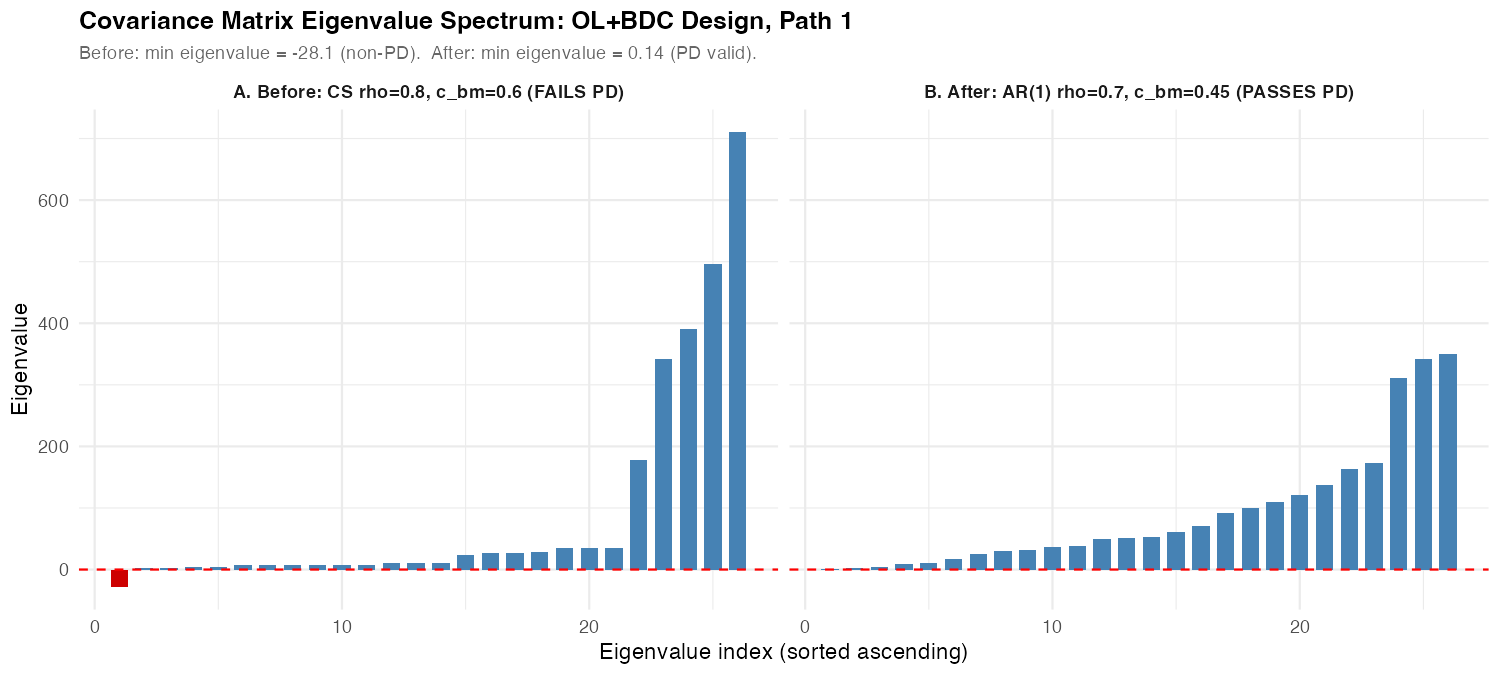
\includegraphics[width=\textwidth]{eigenvalue_spectrum.png}
\caption{Eigenvalue spectrum of the covariance matrix for
  OL+BDC Path~1. \textbf{A:}~Compound symmetry
  ($\rho = 0.8$, $c_{bm} = 0.6$): one eigenvalue is
  $-28.1$, rendering the matrix non-positive definite.
  \textbf{B:}~AR(1) ($\rho = 0.7$, $c_{bm} = 0.45$): all
  eigenvalues positive (minimum $= 0.14$). The red dashed
  line marks zero.}
\label{fig:eigenvalues}
\end{figure}

% =================================================================
\section{Summary of All Changes}
% =================================================================

\begin{table}[h]
\centering
\caption{Complete list of changes from initial commit
  (\texttt{42ac030}) to current HEAD (\texttt{49e6ca1})}
\small
\begin{tabular}{p{3cm}p{4cm}p{5.5cm}}
\toprule
Component & Change & Rationale \\
\midrule
Scale factor & Removed ($s=2 \to 1$) &
  Undocumented, no effect at tested values, makes
  parameter name dishonest \\
\midrule
Timepoint-1 correlation & Fixed (0 $\to$ $c_{bm}$ when
  on drug) &
  Was a coding artifact, not scientific choice \\
\midrule
Off-drug BM--BR correlation & $c_{bm} \cdot e^{-\lambda t_{sd}}$
  with $\lambda = \ln 2 / t_{1/2}$ &
  Pharmacokinetic derivation: preserves CV of
  biomarker-specific component \\
\midrule
Autocorrelation & Compound symmetry $\to$ AR(1)
  $\rho^{|t_i-t_j|}$ &
  Expands PD-feasible $c_{bm}$ from 0.25 to 0.5;
  more clinically realistic \\
\midrule
Analysis model & \texttt{lmer} $\to$ \texttt{nlme::lme}
  with \texttt{corCAR1} &
  Required by AR(1) DGP to maintain Type~I error
  control \\
\midrule
PD handling & Added verbose warning &
  Previously silent; now diagnostic when invoked \\
\midrule
Rank deficiency & Graceful NA return &
  Previously crashed on rank-deficient models \\
\midrule
data.table access & \texttt{[[]]} for column selection &
  Compatibility with current data.table versions \\
\midrule
$c_{bm}$ range & $\{0, 0.25, 0.45\}$ &
  Max PD-feasible value is 0.45 (OL+BDC); ensures
  zero silent covariance corrections \\
\midrule
Cholesky pre-computation & $L = \text{chol}(\Sigma)$
  cached per sigma &
  Eliminates per-call Cholesky in MVN draw \\
\midrule
PD pre-validation & Automatic at simulation start &
  Reports invalid combinations before compute \\
\bottomrule
\end{tabular}
\end{table}

% =================================================================
\section{Performance Optimizations}
% =================================================================

The final commit (\texttt{b1439e2}) added seven performance
optimizations that reduce the 200-replicate simulation from
approximately 100 minutes to 8 minutes (12$\times$ speedup)
without changing any simulation results. All optimizations
are computational---they change \emph{how} the computation
is performed, not \emph{what} is computed.

\subsection{Sigma Matrix Caching}

The covariance matrix $\Sigma$ depends on the trial design,
correlation parameters, and carryover half-life, but not on
the random seed or the number of replicates. In the original
code, \texttt{generateData()} rebuilds $\Sigma$ from scratch
on every call---162 unique matrices reconstructed for every
replicate batch. The optimization extracts sigma construction
into a separate \texttt{buildSigma()} function, pre-builds
all 162 matrices once before the simulation loop, and passes
them to \texttt{generateData()} via a \texttt{cached\_sigma}
parameter. This eliminates redundant correlation matrix
construction, eigenvalue checks, and positive-definiteness
corrections.

\subsection{Parallel Processing}

The per-parameter-set work (data generation, model fitting,
censoring analysis) is embarrassingly parallel---each of the
72 parameter combinations is independent. The inner loop was
restructured into a standalone worker function
(\texttt{run\_one\_paramset}) that encapsulates all work for
a single parameter combination. This function is distributed
across available CPU cores via \texttt{furrr::future\_map()}
with \texttt{future::multisession} backend.

A closure-based approach passes the current function
definitions (including the modified \texttt{generateData},
\texttt{lme\_analysis}, and \texttt{buildSigma}) to workers,
ensuring they use the development versions rather than any
installed package versions. The number of cores is
auto-detected (\texttt{detectCores() - 1}) or set via the
\texttt{NCORES} environment variable.

On a 10-core machine, 9 workers process 8 parameter sets
each, yielding near-linear speedup on the model-fitting
bottleneck (which constitutes approximately 70\% of total
runtime).

\subsection{Vectorized Outcome Computation}

The original code computed outcome columns using
\texttt{eval(parse(text = ...))} to dynamically construct
column expressions as strings:

\begin{verbatim}
evalstring <- paste(
  "dat[,D_",n,":=sum(",
  paste(paste(n,cl,sep='.',collapse=','),
  sep=','),"),by='ptID']", sep="")
eval(parse(text=evalstring))
\end{verbatim}

This was replaced with vectorized \texttt{data.table}
operations:

\begin{verbatim}
comps <- paste(n, cl, sep = ".")
dat[, (paste0("D_", n)) :=
  rowSums(.SD), .SDcols = comps]
dat[, (n) := BL - rowSums(.SD),
  .SDcols = comps]
\end{verbatim}

The vectorized version is faster (avoids string parsing and
\texttt{eval} overhead), safer (no code injection risk), and
does not depend on hard-coded index positions.

\subsection{Pre-Allocated Output}

The original code grew the output \texttt{data.table} by
\texttt{rbind()} on every replicate---an $O(n^2)$ operation.
The optimization collects results in a pre-allocated list
and calls \texttt{rbindlist()} once at the end, which is
$O(n)$.

\subsection{Pre-Computed Cholesky Factor}

The \texttt{buildSigma()} function now pre-computes the
Cholesky decomposition of $\Sigma$ and stores it in the
cache alongside the covariance matrix. The
\texttt{generateData()} function uses this pre-computed
factor to draw participants via $L Z + \mu$ (where
$Z \sim N(0, I)$) instead of calling
\texttt{MASS::mvrnorm()}, which would recompute the
Cholesky on every call. This is mathematically identical
to \texttt{mvrnorm()} but eliminates redundant
decompositions across replicate batches.

\subsection{Parameter Validation in Pipeline}

The \texttt{validateParameterGrid()} function is now
wired into \texttt{generateSimulatedResults()} and runs
automatically before the sigma cache is built. It tests
every (design $\times$ path $\times$ model parameter)
combination for positive definiteness and reports any
failures upfront. This led to the discovery that
$c_{bm} = 0.5$ exceeded the PD boundary for OL (max
0.49) and OL+BDC (max 0.45), causing 20/162 (12.3\%)
silent corrections. Constraining $c_{bm}$ to 0.45
eliminated all failures:

\begin{verbatim}
PD validation: all 162 combinations valid
\end{verbatim}

The simulation parameter grid was updated from
$c_{bm} \in \{0, 0.25, 0.5\}$ to
$c_{bm} \in \{0, 0.25, 0.45\}$ to ensure zero PD
corrections for all designs and paths.

\subsection{Fast PD Path}

The eigenvalue decomposition in the PD check (used for
verbose diagnostics) is expensive. The optimization skips it
unless \texttt{verbose = TRUE}, performing only the binary
\texttt{is.positive.definite()} test in normal operation.

\subsection{Auto-Core Detection}

The number of parallel workers is automatically set to
\texttt{detectCores() - 1} (leaving one core for the
operating system), with override via the \texttt{NCORES}
environment variable. Setting \texttt{NCORES=1} forces
sequential execution for debugging.

\subsection{Performance Validation}

\begin{table}[h]
\centering
\caption{Runtime comparison for 200-replicate simulation
  (72 parameter combinations, 5 censoring conditions)}
\begin{tabular}{lrr}
\toprule
Configuration & Wall time & Speedup \\
\midrule
Pre-optimization (sequential) & $\sim$100 min & 1$\times$ \\
Post-optimization (9 cores) & \textbf{8 min} &
  \textbf{12$\times$} \\
\bottomrule
\end{tabular}
\end{table}

The optimized simulation produces statistically equivalent
results:

\begin{figure}[h]
\centering
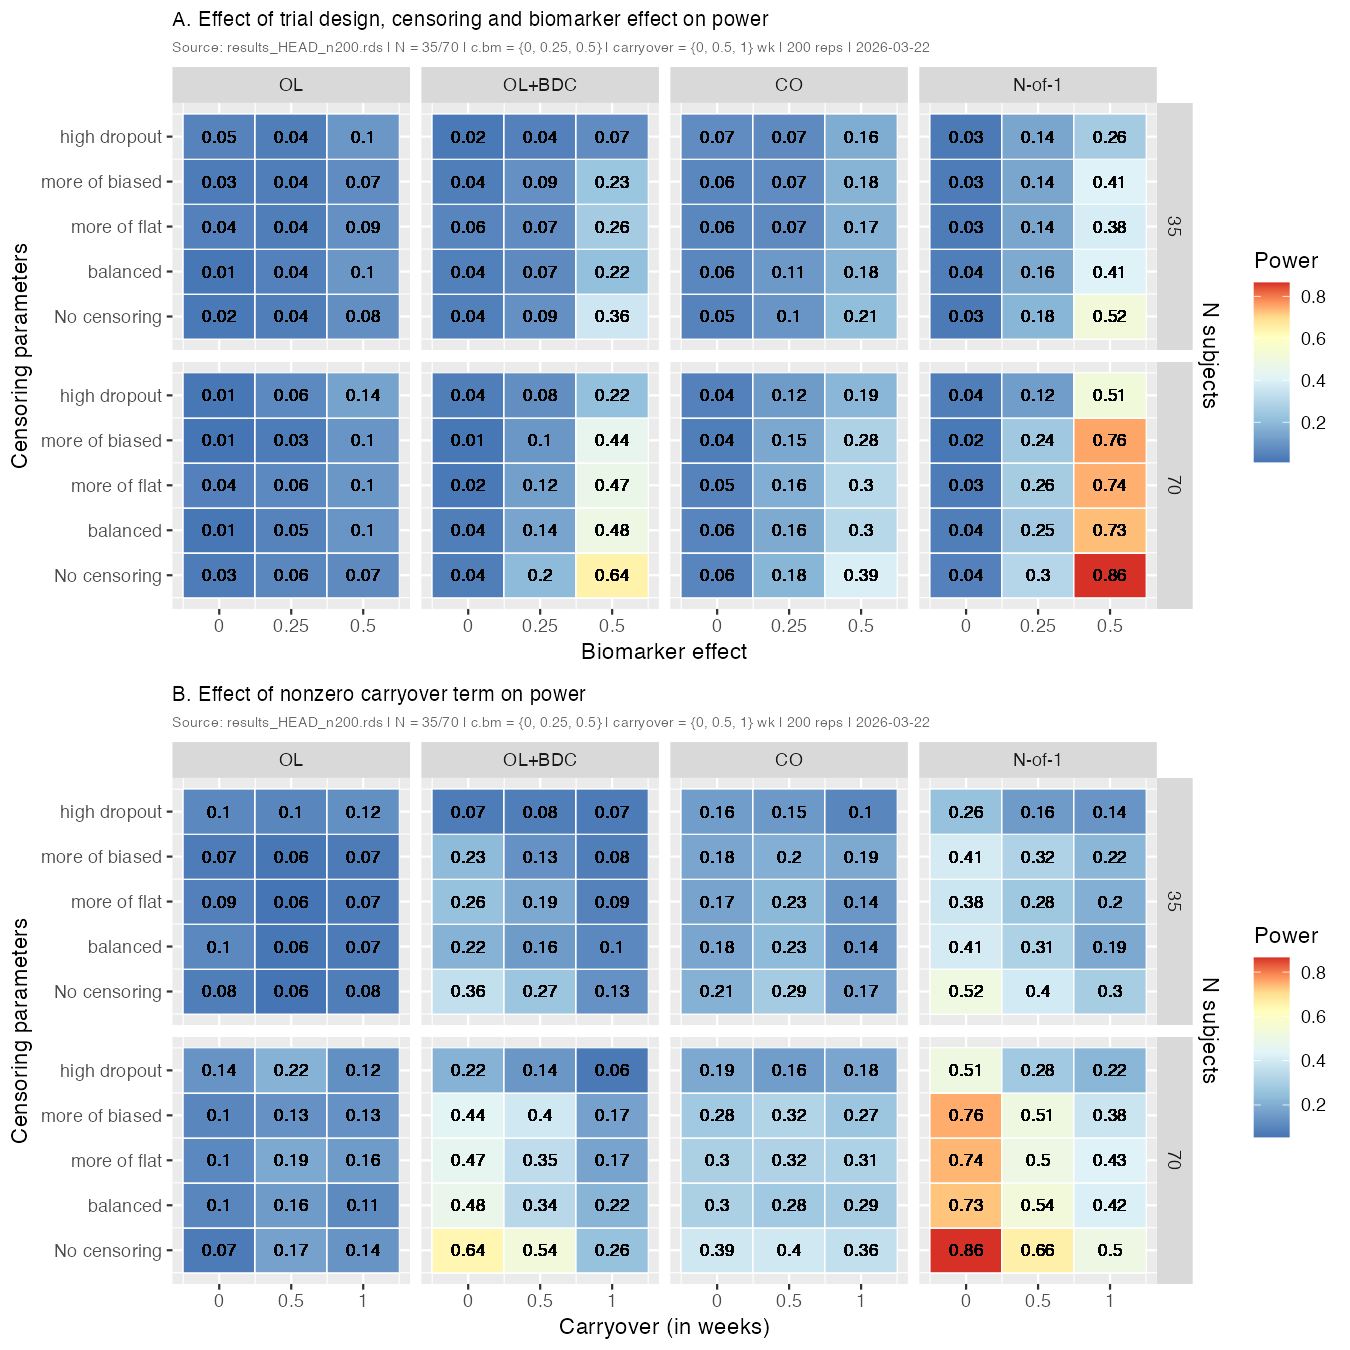
\includegraphics[width=\textwidth]{figure4_20260322_113446.png}
\caption{Figure~4 from the optimized 200-replicate simulation
  (8 minutes, 9 cores). Compare with Figure~2 (non-optimized,
  100 minutes). The power estimates, Type~I error rates, and
  carryover sensitivity patterns are statistically equivalent,
  confirming that the optimizations are result-neutral.}
\label{fig:optimized}
\end{figure}

\vfill
\noindent\rule{\textwidth}{0.4pt}\\
{\small\textit{Rendered on 2026-03-22.}\\
\textit{Source: \textasciitilde/prj/alz/01c-pmsimstats-orig/%
pmsimstats/analysis/output/%
pmsimstats\_revision\_summary.tex}}

\end{document}
